% ----------------------------------------------------------------- %
%             The Speech Signal Processing Toolkit (SPTK)           %
%             developed by SPTK Working Group                       %
%             http://sp-tk.sourceforge.net/                         %
% ----------------------------------------------------------------- %
%                                                                   %
%  Copyright (c) 1984-2007  Tokyo Institute of Technology           %
%                           Interdisciplinary Graduate School of    %
%                           Science and Engineering                 %
%                                                                   %
%                1996-2016  Nagoya Institute of Technology          %
%                           Department of Computer Science          %
%                                                                   %
% All rights reserved.                                              %
%                                                                   %
% Redistribution and use in source and binary forms, with or        %
% without modification, are permitted provided that the following   %
% conditions are met:                                               %
%                                                                   %
% - Redistributions of source code must retain the above copyright  %
%   notice, this list of conditions and the following disclaimer.   %
% - Redistributions in binary form must reproduce the above         %
%   copyright notice, this list of conditions and the following     %
%   disclaimer in the documentation and/or other materials provided %
%   with the distribution.                                          %
% - Neither the name of the SPTK working group nor the names of its %
%   contributors may be used to endorse or promote products derived %
%   from this software without specific prior written permission.   %
%                                                                   %
% THIS SOFTWARE IS PROVIDED BY THE COPYRIGHT HOLDERS AND            %
% CONTRIBUTORS "AS IS" AND ANY EXPRESS OR IMPLIED WARRANTIES,       %
% INCLUDING, BUT NOT LIMITED TO, THE IMPLIED WARRANTIES OF          %
% MERCHANTABILITY AND FITNESS FOR A PARTICULAR PURPOSE ARE          %
% DISCLAIMED. IN NO EVENT SHALL THE COPYRIGHT OWNER OR CONTRIBUTORS %
% BE LIABLE FOR ANY DIRECT, INDIRECT, INCIDENTAL, SPECIAL,          %
% EXEMPLARY, OR CONSEQUENTIAL DAMAGES (INCLUDING, BUT NOT LIMITED   %
% TO, PROCUREMENT OF SUBSTITUTE GOODS OR SERVICES; LOSS OF USE,     %
% DATA, OR PROFITS; OR BUSINESS INTERRUPTION) HOWEVER CAUSED AND ON %
% ANY THEORY OF LIABILITY, WHETHER IN CONTRACT, STRICT LIABILITY,   %
% OR TORT (INCLUDING NEGLIGENCE OR OTHERWISE) ARISING IN ANY WAY    %
% OUT OF THE USE OF THIS SOFTWARE, EVEN IF ADVISED OF THE           %
% POSSIBILITY OF SUCH DAMAGE.                                       %
% ----------------------------------------------------------------- %
\hypertarget{phase}{}
\name{phase}{transform real sequence to phase}{signal processing}

\begin{synopsis}
\item[phase] [ --l $L$ ] [ --p {\em pfile} ] [ --z {\em zfile} ]
             [ --m $M$ ] [ --n $N$ ] [ --u ] [ {\em infile} ]
\end{synopsis}

\begin{qsection}{DESCRIPTION}
{\em phase} calculates the phase of the spectrum of a real sequence 
from {\em infile} (or standard input), 
and sends the result to standard output.
Assume that the input sequence is
\begin{displaymath}
  x(0), x(1), \dots, x(L-1)
\end{displaymath}
and the FFT is
\begin{align}
  X_k &= X(e^{j\omega}) \left|
	\begin{array}{c}
	\\
        \omega=\frac{2\pi k}{L}
	\end{array}
    \right. \notag \\
         &= \sum_{m=0}^{L-1}x(m)e^{-j\omega m} \left|
	\begin{array}{c}
	\\
        \omega=\frac{2\pi\, k}{L}
	\end{array}
    \right.,\qquad k=0,1,\dots,L-1 \notag
\end{align}
Then the output is given by
\begin{displaymath}
  Y_k=\arg X_k, \qquad k=0,1,\dots,L/2
\end{displaymath}
In this case the phase is written in continuous form.
The output data angular frequency varies from $0\sim \pi$.
Input and output data are in float format.
\par
If the {\bf --p, --z} options are assigned
then the phase of the corresponding filter related to
the assigned coefficients is calculated
\footnote{
In this case the phase is not evaluated from the filter
impulse response, but from
the difference between the numerator and denominator phases}.
\end{qsection}

\begin{options}
    \argm{l}{L}{frame length power of 2}{256}
    \argm{p}{pfile}{numerator coefficients file\\
            The {\em pfile} should follow this structure in
            float format:\\
            \hspace*{2ex}$K, a(1), \dots, a(M)$\\[-1ex]}{NULL}
    \argm{z}{zfile}{denominator coefficients file\\
            The {\em zfile} should follow this structure in
            float format:\\
            \hspace*{2ex}$b(0), b(1), \dots, b(N)$\\
            The contents of {\em pfile} and {\em zfile}
            should be in a similar form to that used in
            the {\em dfs} command.
            When only the {\bf --p} option is assigned
            then the denominator is made equal to 1.
            When only the {\bf --z} option is assigned,
            the numerator and the gain $K$ are both set to 1.
            If neither {\bf --p} nor {\bf --z} are
            assigned, data is read from the standard input.}{NULL}
    \argm{m}{M}{order of polynomial denominator\\
            If the number of input data
            values is less $M+1$, then $M$ is set to the number
            of input data values $-1$.
            On the other hand, There is no need to assign a values to
            $M$ if one doesn't want the data to be analyzed is
            blocks of $M+1$ size.}{$L-1$}
    \argm{n}{N}{order of polynomial numerator\\
            Likewise the --m option,
            if the number of input data
            values is less then $N+1$, then $N$ is set
            to the number of input data values $-1$.
            On the other hand, There is no need to assign a values to
            $N$ if one doesn't want the data to be analyzed is
            blocks of $N+1$ size.}{$L-1$}
    \argm{u}{}{unwrapping}{TRUE}
\end{options}

\begin{qsection}{EXAMPLE}
In the example below, the phase characteristic of a digital filter
with coefficients assigned by the files {\em data.p, data.z} 
in float format can be displayed by:
\begin{quote}
  \verb!phase -p data.p -z data.z | fdrw | xgr !
\end{quote}
\begin{center}
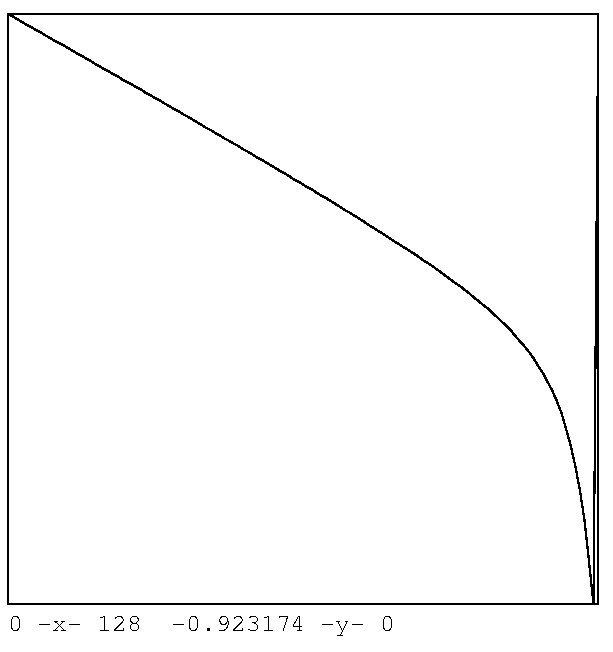
\includegraphics[width=6cm]{fig/phase_1.pdf}
\end{center}
If the filter defined by {\em data.p}, {\em data.z} is stable
then the following command will give a similar result:
\begin{quote}
  \verb!impulse | dfs -p data.p -z data.z | phase | fdrw | xgr !
\end{quote}
\begin{center}
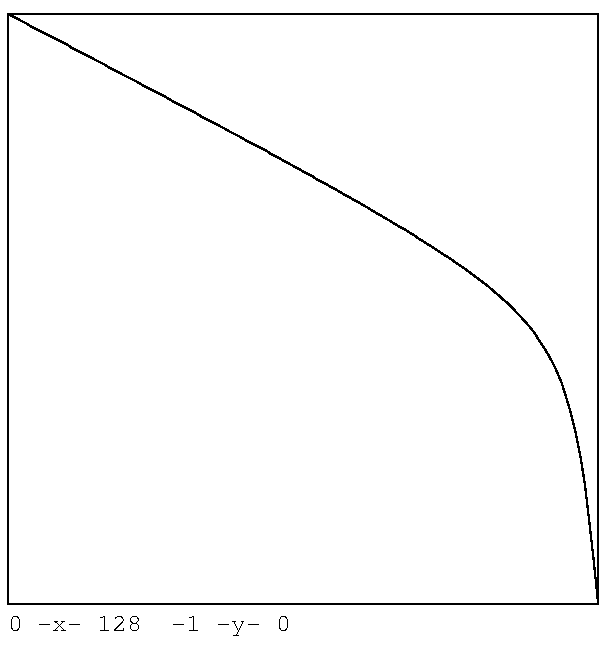
\includegraphics[width=6cm]{fig/phase_2.pdf}
\end{center}
\end{qsection}

\begin{qsection}{SEE ALSO}
\hyperlink{spec}{spec},
\hyperlink{fft}{fft},
\hyperlink{fftr}{fftr},
\hyperlink{dfs}{dfs}
\end{qsection}

\begin{qsection}{NOTICE}
If the sample interval between FFT points is large
(the value assigned by the --l option is small),
or if the phase characteristic includes steep angles
(i.e. zeros and/or poles are close to the unit circle in the $z$
 domain), it might happen that the phase is not properly drawn in continuous form.
\end{qsection}
